\documentclass[11pt,a4paper]{article}

\usepackage[T1]{fontenc}
\usepackage[utf8]{inputenc}
\usepackage[scaled=0.95]{helvet}
\usepackage{courier}
\usepackage{microtype}
\DisableLigatures[-]{encoding = *, family = tt*}
\usepackage[a4paper,left=2cm,right=2cm,top=2.3cm,bottom=2.2cm]{geometry}
\usepackage[table]{xcolor}
\usepackage{tikz}
\usetikzlibrary{arrows.meta,positioning,fit,backgrounds,calc,shapes.geometric,decorations.pathreplacing}
\usepackage[most]{tcolorbox}
\usepackage{listings}
\usepackage{booktabs,tabularx,array}
\usepackage{enumitem}
\usepackage{titlesec}
\usepackage{fancyhdr}
\usepackage{url}
\usepackage{longtable}
\usepackage{needspace}
\DeclareUrlCommand{\f}{\urlstyle{tt}}
\usepackage[colorlinks=true,linkcolor=azure,urlcolor=azure,citecolor=azure,pdftitle={PipeDoctor - Step 2 decoded},pdfauthor={PipeDoctor project}]{hyperref}

\renewcommand{\familydefault}{\sfdefault}
\setlength{\parindent}{0pt}
\setlength{\parskip}{5pt}
\emergencystretch=2em
\renewcommand{\arraystretch}{1.25}

% ---------- colours ----------
\definecolor{navy}{HTML}{1F3A5F}
\definecolor{azure}{HTML}{0B6FB8}
\definecolor{teal}{HTML}{1F8A80}
\definecolor{bronze}{HTML}{B07A3A}
\definecolor{silver}{HTML}{7F8B98}
\definecolor{gold}{HTML}{C9A227}
\definecolor{alert}{HTML}{C0392B}
\definecolor{ok}{HTML}{2E8B57}
\definecolor{amber}{HTML}{D98A00}
\definecolor{codebg}{HTML}{F3F6F9}
\definecolor{rowgray}{HTML}{F4F6F8}

% ---------- headings ----------
\titleformat{\section}{\Large\bfseries\color{navy}}{\thesection}{0.6em}{}[\vspace{-0.2em}{\color{navy!35}\titlerule[0.8pt]}]
\titleformat{\subsection}{\large\bfseries\color{azure}}{\thesubsection}{0.5em}{}
\titlespacing*{\section}{0pt}{16pt}{7pt}
\titlespacing*{\subsection}{0pt}{10pt}{3pt}

% ---------- header / footer ----------
\pagestyle{fancy}
\fancyhf{}
\renewcommand{\headrulewidth}{0.3pt}
\fancyhead[L]{\small\color{navy}\textbf{PipeDoctor} \textperiodcentered\ Step 2 decoded}
\fancyhead[R]{\small\color{silver}Sprint 1 \textperiodcentered\ run of 8 Oct 2026}
\fancyfoot[C]{\small\color{silver}\thepage}

% ---------- helpers ----------
\newcommand{\figcap}[1]{\par\smallskip{\centering\small #1\par}}
\let\oldsection\section
\renewcommand{\section}{\Needspace*{9\baselineskip}\oldsection}
\newcommand{\badge}[1]{\tikz[baseline=(b.base)]\node[circle,fill=azure,text=white,inner sep=0pt,minimum size=13pt,font=\bfseries\scriptsize] (b) {#1};}
\newcommand{\sub}[1]{\par\vspace{2pt}{\bfseries\color{navy}#1}\par\vspace{-2pt}}
\newcommand{\fl}[2]{\f{#1}\,{\color{silver}(#2)}}

\tcbset{
  boxbase/.style={enhanced,breakable,left=8pt,right=8pt,top=5pt,bottom=5pt,boxrule=0pt,
    frame hidden,arc=3pt,fontupper=\small,before skip=6pt,after skip=8pt},
}
\newtcolorbox{goal}[1][]{boxbase,colback=azure!8,borderline west={3pt}{0pt}{azure},title={},#1}
\newtcolorbox{good}[1][]{boxbase,colback=ok!10,borderline west={3pt}{0pt}{ok},#1}
\newtcolorbox{watch}[1][]{boxbase,colback=amber!12,borderline west={3pt}{0pt}{amber},#1}
\newtcolorbox{pd}[1][]{boxbase,colback=navy!7,borderline west={3pt}{0pt}{navy},#1}

% ---------- listings ----------
\lstdefinelanguage{docker}{morekeywords={FROM,RUN,COPY,WORKDIR,ENV},sensitive=true,morecomment=[l]{\#}}
\lstdefinestyle{code}{
  basicstyle=\ttfamily\footnotesize,backgroundcolor=\color{codebg},
  numbers=left,numberstyle=\ttfamily\scriptsize\color{navy!55},numbersep=8pt,
  frame=l,framerule=2pt,rulecolor=\color{azure},xleftmargin=30pt,framexleftmargin=27pt,
  aboveskip=5pt,belowskip=6pt,showstringspaces=false,
  keywordstyle=\color{azure}\bfseries,commentstyle=\color{silver}\itshape,
  stringstyle=\color{teal},breaklines=true,columns=fullflexible,keepspaces=true,
  upquote=true}
\lstdefinestyle{out}{
  language={},numbers=none,basicstyle=\ttfamily\footnotesize,backgroundcolor=\color{rowgray},
  frame=l,framerule=2pt,rulecolor=\color{silver},xleftmargin=8pt,framexleftmargin=6pt,
  aboveskip=5pt,belowskip=6pt,showstringspaces=false,breaklines=true,columns=fullflexible,keepspaces=true}
\lstdefinestyle{cmd}{
  language={},numbers=none,basicstyle=\ttfamily\footnotesize,backgroundcolor=\color{navy!8},
  frame=l,framerule=2pt,rulecolor=\color{navy},xleftmargin=8pt,framexleftmargin=6pt,
  aboveskip=5pt,belowskip=6pt,breaklines=true,columns=fullflexible,keepspaces=true,
  prebreak=\mbox{\textbackslash}}

% numbered file excerpt: \code{python}{first line}
\newcommand{\codestyle}[2]{\lstset{style=code,language=#1,firstnumber=#2}}

\begin{document}
\sloppy

% =============================== TITLE ===============================
\begin{tcolorbox}[enhanced,colback=navy,colframe=navy,arc=4pt,boxrule=0pt,left=14pt,right=14pt,top=12pt,bottom=12pt]
{\color{white}
{\Huge\bfseries PipeDoctor\\[2pt]Step 2, decoded}\\[8pt]
{\large What your first Docker run really did, in 7 steps,\\ with the files and lines of code behind each one.}\\[10pt]
{\small Sprint 1 \textperiodcentered\ Step 2 (local lakehouse) \textperiodcentered\ run of Thursday 8 October 2026\\
Read it next to \f{docs/guide/02-code-walkthrough.md} and keep VS Code open on the code.}}
\end{tcolorbox}

\begin{good}
\textbf{Your run is green.} Raw taxi files went in; three Delta tables came out; the second run changed nothing.\par\smallskip
\begin{itemize}[leftmargin=14pt,itemsep=1pt,topsep=2pt]
\item \textbf{It works:} 8 of 8 tests pass. 9\,554\,778 raw rows $\rightarrow$ 9\,417\,635 clean trips + 137\,142 quarantined $\rightarrow$ 20\,623 gold rows.
\item \textbf{It is safe to re-run} (idempotent): run 2 skipped the 3 files already loaded, added 0 rows to silver, and printed the same counts.
\end{itemize}
This is exactly the healthy baseline PipeDoctor needs: a pipeline that works, that we understand, and that we can break on purpose later.
\end{good}

% =============================== 1 PICTURE ===============================
\section{The whole picture on one page}

\begin{figure}[h]
\centering
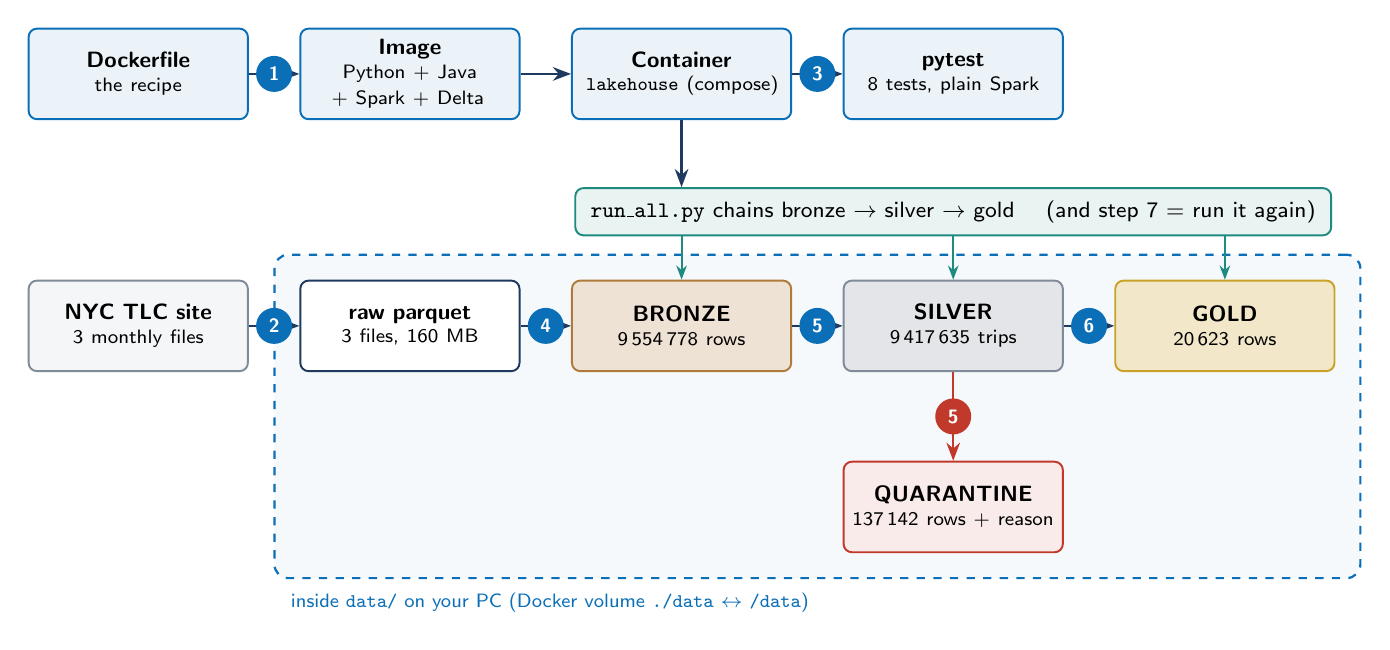
\begin{tikzpicture}[
  font=\footnotesize,
  box/.style={draw=navy,rounded corners=3pt,fill=white,minimum height=1.15cm,text width=2.55cm,align=center,line width=0.7pt},
  ext/.style={box,draw=silver,fill=rowgray},
  bronze/.style={box,draw=bronze,fill=bronze!22},
  silver/.style={box,draw=silver,fill=silver!22},
  gold/.style={box,draw=gold,fill=gold!25},
  quar/.style={box,draw=alert,fill=alert!10},
  infra/.style={box,draw=azure,fill=azure!8},
  arr/.style={-{Stealth[length=2.3mm]},line width=0.9pt,color=navy},
  bd/.style={circle,fill=azure,text=white,inner sep=0pt,minimum size=13pt,font=\bfseries\scriptsize}
]
% ---- row 1: infrastructure ----
\node[infra] (df)  at (0,3.2)    {\textbf{Dockerfile}\\[-1pt]\scriptsize the recipe};
\node[infra] (img) at (3.45,3.2) {\textbf{Image}\\[-1pt]\scriptsize Python + Java + Spark + Delta};
\node[infra] (ct)  at (6.9,3.2)  {\textbf{Container}\\[-1pt]\scriptsize \texttt{lakehouse} (compose)};
\node[infra] (pt)  at (10.35,3.2){\textbf{pytest}\\[-1pt]\scriptsize 8 tests, plain Spark};
\draw[arr] (df) -- node[bd,fill=azure] {1} (img);
\draw[arr] (img) -- (ct);
\draw[arr] (ct) -- node[bd] {3} (pt);
% ---- run_all bar ----
\node[draw=teal,fill=teal!10,rounded corners=3pt,minimum height=0.6cm,minimum width=9.6cm,line width=0.7pt]
  (ra) at (10.35,1.45) {\texttt{run\_all.py} chains bronze $\rightarrow$ silver $\rightarrow$ gold \quad(and step 7 = run it again)};
\draw[arr] (ct.south) -- (ct.south |- ra.north);
% ---- row 2: data ----
\node[ext]    (tlc) at (0,0)     {\textbf{NYC TLC site}\\[-1pt]\scriptsize 3 monthly files};
\node[box]    (raw) at (3.45,0)  {\textbf{raw parquet}\\[-1pt]\scriptsize 3 files, 160 MB};
\node[bronze] (br)  at (6.9,0)   {\textbf{BRONZE}\\[-1pt]\scriptsize 9\,554\,778 rows};
\node[silver] (si)  at (10.35,0) {\textbf{SILVER}\\[-1pt]\scriptsize 9\,417\,635 trips};
\node[gold]   (go)  at (13.8,0)  {\textbf{GOLD}\\[-1pt]\scriptsize 20\,623 rows};
\node[quar]   (qu)  at (10.35,-2.3){\textbf{QUARANTINE}\\[-1pt]\scriptsize 137\,142 rows + reason};
\draw[arr] (tlc) -- node[bd] {2} (raw);
\draw[arr] (raw) -- node[bd] {4} (br);
\draw[arr] (br)  -- node[bd] {5} (si);
\draw[arr] (si)  -- node[bd] {6} (go);
\draw[arr,color=alert] (si) -- node[bd,fill=alert] {5} (qu);
% ticks from run_all
\foreach \n in {br,si,go} {\draw[teal,line width=0.7pt,-{Stealth[length=1.8mm]}] (\n |- ra.south) -- (\n.north);}
% volume enclosure
\begin{scope}[on background layer]
\node[draw=azure,dashed,rounded corners=5pt,fill=azure!4,line width=0.8pt,fit=(raw)(br)(si)(go)(qu),inner sep=9pt] (vol) {};
\end{scope}
\node[font=\scriptsize,text=azure,anchor=north west] at ($(vol.south west)+(0.1,-0.05)$) {inside \texttt{data/} on your PC (Docker volume \texttt{./data} $\leftrightarrow$ \texttt{/data})};
\end{tikzpicture}
\figcap{\textbf{Figure 1.} The seven numbered steps. Blue = tooling (steps 1 and 3), grey = outside world, coloured = the data layers. Step 7 is step 4--6 run a second time.}
\end{figure}

\subsection*{Six words you will hear all project long}
\rowcolors{2}{rowgray}{white}
\begin{longtable}{@{}>{\bfseries}p{2.3cm}p{7.9cm}p{5.8cm}@{}}
\toprule
Word & In plain words & Where it lives \\
\midrule
\endhead
Image & A frozen computer set-up (Python, Java, Spark, Delta) built once from a recipe. & \f{docker/Dockerfile} \\
Container & A running copy of the image. Our commands run \emph{inside} it; with \texttt{--rm} it is deleted afterwards. & started by \f{docker-compose.yml} \\
Volume & A folder shared between your PC and the container, so files survive after the container is gone. & \f{docker-compose.yml} lines 7--9 \\
Delta table & Parquet files plus a \f{_delta_log/} folder that records every change. This gives us history, constraints and MERGE. & \f{data/lakehouse/...} \\
Medallion & Bronze = raw as received, silver = clean and typed, gold = business view. & \f{pipelines/*.py} \\
Idempotent & Run it twice, get the same result. Retries become safe. & \f{bronze.py} line 33, \f{silver.py} line 36 \\
\bottomrule
\end{longtable}

% =============================== 2 AT A GLANCE ===============================
\section{The 7 steps at a glance}
\rowcolors{2}{rowgray}{white}
\begin{tabularx}{\textwidth}{@{}c>{\bfseries\raggedright\arraybackslash}p{3.0cm}p{6.1cm}X@{}}
\toprule
\# & Step & Code that does the work & What your output showed \\
\midrule
1 & Build the image & \f{docker/Dockerfile}, \f{docker/requirements.txt} & \texttt{Image pipedoctor-lakehouse Built 150.2s} \\
2 & Download the data & \f{scripts/download_taxi_data.py} & 3 files: 50.0 + 50.3 + 60.1 MB \\
3 & Unit tests & \f{pipelines/tests/test_transforms.py} & \texttt{8 passed in 34.78s} \\
4 & Bronze & \f{pipelines/bronze.py}, \f{transforms.py:61} & \texttt{9,554,778 rows in bronze} \\
5 & Silver & \f{pipelines/silver.py}, \f{transforms.py:73-149} & \texttt{9,417,635 trips, 137,142 quarantined} \\
6 & Gold & \f{pipelines/gold.py}, \f{transforms.py:152} & \texttt{20,623 rows}, \texttt{green in 567s} \\
7 & Re-run (idempotence) & same code, skip and MERGE logic & same counts, \texttt{green in 134s} \\
\bottomrule
\end{tabularx}

\medskip
\textbf{Careful with the word ``step''.} The numbers 1--7 in this document are the seven stages of \emph{this run}. The sprint plan has its own steps (Step 3 = GitHub and CI, and so on).

You typed only \textbf{five different commands}; steps 4, 5 and 6 are one command (\texttt{run\_all}), and step 7 is that same command a second time. The extra \texttt{pytest} run in your log is a repeat of step 3 and proves nothing new.

% =============================== STEP 1 ===============================
\section{Step 1 \textemdash\ Build the image}
\begin{goal}\textbf{Goal.} Build a reusable ``box'' holding everything the pipeline needs, so it runs identically on your PC, in GitHub CI later, and in PipeDoctor's sandbox.\end{goal}

\sub{Command}
\begin{lstlisting}[style=cmd]
docker compose build
\end{lstlisting}
\f{docker-compose.yml:3-5} tells Compose to build from \f{docker/Dockerfile} using the project folder as context.

\sub{Code behind it \textemdash\ and the answer to ``is this automated?''}
No magic and no hidden script: the \textbf{Dockerfile is our own recipe}. Docker runs it line by line, and each instruction becomes one cached \emph{layer} (your log shows \texttt{[1/6]} to \texttt{[6/6]}). The commands \emph{inside} the layers (\texttt{apt-get}, \texttt{pip}) are standard tools.

\codestyle{docker}{4}
\begin{lstlisting}
RUN apt-get update \
 && apt-get install -y --no-install-recommends openjdk-17-jre-headless procps \
 && rm -rf /var/lib/apt/lists/*

COPY docker/requirements.txt /tmp/requirements.txt
RUN pip install --no-cache-dir -r /tmp/requirements.txt
\end{lstlisting}

\begin{itemize}[leftmargin=14pt,itemsep=1pt]
\item \fl{Dockerfile}{line 2}: start from the official slim Debian + Python 3.11 image (log \texttt{\#7}, 18.9\,s: layers downloaded).
\item \fl{Dockerfile}{lines 4--6}: install \textbf{Java 17}. Spark runs on the JVM; ``PySpark'' is only the Python remote control. 27 packages, 53.8\,MB (log \texttt{\#8}, 22.2\,s).
\item \fl{Dockerfile}{lines 8--9}: install the \textbf{pinned} versions of \f{docker/requirements.txt}: \texttt{pyspark==3.5.3}, \texttt{delta-spark==3.2.1}, \texttt{pytest==8.3.3}. Pinned because Delta 3.2 is built for Spark 3.5; mixing versions gives cryptic Java errors (log \texttt{\#10}, 61.2\,s, PySpark alone is 317\,MB).
\end{itemize}

\codestyle{docker}{11}
\begin{lstlisting}
# Pre-fetch the Delta jars at build time so runs do not need internet for them.
RUN python -c "\
from delta import configure_spark_with_delta_pip as c; \
from pyspark.sql import SparkSession as S; \
b = (S.builder.master('local[1]') \
     .config('spark.sql.extensions','io.delta.sql.DeltaSparkSessionExtension') \
     .config('spark.sql.catalog.spark_catalog','org.apache.spark.sql.delta.catalog.DeltaCatalog')); \
s = c(b).getOrCreate(); s.range(1).write.format('delta').save('/tmp/warmup'); s.stop()"
\end{lstlisting}
\begin{itemize}[leftmargin=14pt,itemsep=1pt]
\item \fl{Dockerfile}{lines 11--18}: the \textbf{warm-up}. It starts Spark once and writes a 1-row Delta table so the three Delta jars are downloaded \emph{now} (log \texttt{\#11}: \texttt{downloading ... delta-spark\_2.12-3.2.1.jar}, 13.9\,s). \textbf{Proof it worked:} in the later runs the log says \texttt{0 artifacts copied, 3 already retrieved}.
\end{itemize}

\codestyle{docker}{20}
\begin{lstlisting}
WORKDIR /workspace
ENV PYTHONPATH=/workspace \
    PYTHONUNBUFFERED=1 \
    LAKEHOUSE_DIR=/data/lakehouse \
    RAW_DIR=/data/raw
\end{lstlisting}
\begin{itemize}[leftmargin=14pt,itemsep=1pt]
\item \fl{Dockerfile}{lines 20--24}: \texttt{PYTHONPATH} lets \texttt{import pipelines} work; \texttt{LAKEHOUSE\_DIR} and \texttt{RAW\_DIR} are read by \f{pipelines/common/spark.py:5-6} to know where the data lives.
\end{itemize}

\begin{figure}[h]
\centering
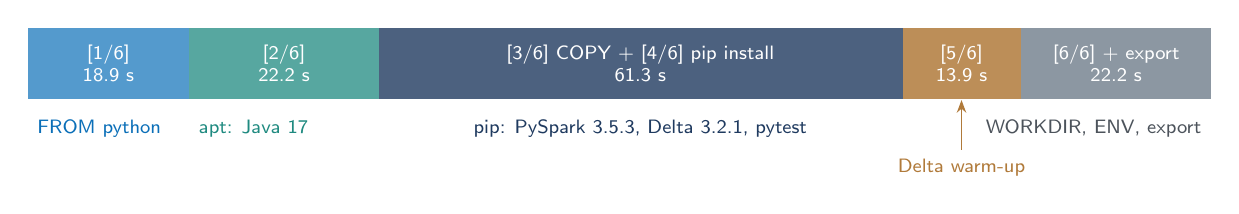
\begin{tikzpicture}[font=\scriptsize]
\def\s{0.1085}
\def\h{0.9}
\fill[azure!70]   (0,0)                 rectangle ++(18.9*\s,\h);
\fill[teal!75]    (18.9*\s,0)           rectangle ++(22.2*\s,\h);
\fill[navy!80]    (41.1*\s,0)           rectangle ++(61.3*\s,\h);
\fill[bronze!85]  (102.4*\s,0)          rectangle ++(13.9*\s,\h);
\fill[silver!90]  (116.3*\s,0)          rectangle ++(22.2*\s,\h);
\node[white,align=center] at (9.45*\s,\h/2)   {[1/6]\\18.9 s};
\node[white,align=center] at (30*\s,\h/2)     {[2/6]\\22.2 s};
\node[white,align=center] at (71.7*\s,\h/2)   {[3/6] COPY + [4/6] pip install\\61.3 s};
\node[white,align=center] at (109.3*\s,\h/2)  {[5/6]\\13.9 s};
\node[white,align=center] at (127.4*\s,\h/2)  {[6/6] + export\\22.2 s};
\node[anchor=north west,text=azure]   at (0,-0.15)             {FROM python};
\node[anchor=north west,text=teal]    at (18.9*\s,-0.15)       {apt: Java 17};
\node[anchor=north,text=navy]         at (71.7*\s,-0.15)       {pip: PySpark 3.5.3, Delta 3.2.1, pytest};
\node[anchor=north,text=bronze]       at (109.3*\s,-0.65)      {Delta warm-up};
\node[anchor=north east,text=silver!60!black] at (138.5*\s,-0.15) {WORKDIR, ENV, export};
\draw[-{Stealth[length=1.6mm]},line width=0.5pt,bronze] (109.3*\s,-0.65) -- (109.3*\s,-0.02);
\end{tikzpicture}
\figcap{\textbf{Figure 2.} Where the 150\,s of \texttt{docker compose build} went (bar widths proportional to time). Pip is the slowest layer; a second build reuses every cached layer and takes seconds.}
\end{figure}

\sub{Why it matters for PipeDoctor}
Rebuild only when \texttt{Dockerfile} or \texttt{requirements.txt} change. When the agent later runs a candidate fix in its sandbox, it will use this same image, so ``it works in the sandbox'' means ``it works here''.

% =============================== STEP 2 ===============================
\section{Step 2 \textemdash\ Download the data}
\begin{goal}\textbf{Goal.} Get real data: three months (Jan--Mar 2024) of NYC yellow-taxi trips, about 9.5 million rows.\end{goal}

\sub{Command}
\begin{lstlisting}[style=cmd]
docker compose run --rm lakehouse python scripts/download_taxi_data.py --start 2024-01 --months 3
\end{lstlisting}
\texttt{compose run} starts a \emph{new container} from the image, mounts your project as \texttt{/workspace} and \texttt{./data} as \texttt{/data} (\f{docker-compose.yml:7-9}), runs the command, and \texttt{--rm} deletes the container afterwards. The files stay on your PC in \f{data/raw/yellow/}.

\sub{Code behind it}
\codestyle{python}{29}
\begin{lstlisting}
    for ym in month_range(a.start, a.months):
        dest = os.path.join(a.out, f"yellow_tripdata_{ym}.parquet")
        if os.path.exists(dest):
            print(f"skip   {dest} (already there)")
            continue
        url = BASE.format(ym=ym)
        print(f"get    {url}")
        tmp = dest + ".part"
        urllib.request.urlretrieve(url, tmp)
        os.replace(tmp, dest)
        print(f"saved  {dest} ({os.path.getsize(dest) / 1e6:.1f} MB)")
\end{lstlisting}
\begin{itemize}[leftmargin=14pt,itemsep=1pt]
\item \fl{scripts/download_taxi_data.py}{line 10}: \texttt{BASE} is the public CloudFront address of the TLC files, one file per month.
\item Lines 31--33: \textbf{skip if present}, so running twice never downloads twice.
\item Lines 36--38: download to \texttt{*.part}, then \texttt{os.replace} renames it. A file that exists under its real name is therefore always complete.
\end{itemize}

\sub{What your output showed}
\begin{lstlisting}[style=out]
saved  /data/raw/yellow/yellow_tripdata_2024-01.parquet (50.0 MB)
saved  /data/raw/yellow/yellow_tripdata_2024-02.parquet (50.3 MB)
saved  /data/raw/yellow/yellow_tripdata_2024-03.parquet (60.1 MB)
\end{lstlisting}
160.4\,MB in total. The line \texttt{Network pipedoctor\_default Created} is Compose making a private network; we do not use it.

\sub{Why it matters for PipeDoctor}
File-arrival problems come later (a \emph{late} file is failure scenario 4, which PipeDoctor must escalate rather than patch). The \texttt{.part} rename is what guarantees that a visible file is a complete one.

% =============================== STEP 3 ===============================
\section{Step 3 \textemdash\ Unit tests}
\begin{goal}\textbf{Goal.} Prove the transformation logic is correct on tiny hand-made tables \emph{before} spending minutes on 9.5 million rows.\end{goal}

\sub{Command}
\begin{lstlisting}[style=cmd]
docker compose run --rm lakehouse python -m pytest pipelines/tests -q
\end{lstlisting}
\texttt{-q} means quiet: one dot per passing test. Your output, \texttt{........ 8 passed in 34.78s}, is 8 dots = 8 tests. The 35\,s is mostly Spark starting its Java engine; the repeat took 18\,s.

\sub{Code behind it}
\codestyle{python}{6}
\begin{lstlisting}
@pytest.fixture(scope="session")
def spark():
    s = get_spark("tests", delta=False)  # transforms are tested without Delta
    yield s
    s.stop()
\end{lstlisting}
\fl{pipelines/tests/conftest.py}{lines 6--10}: one Spark session shared by all tests, \emph{without} Delta (\f{pipelines/common/spark.py:24} only loads Delta when \texttt{delta=True}). Possible because the transforms are pure DataFrame-in, DataFrame-out functions (\f{transforms.py:1}).

\rowcolors{2}{rowgray}{white}
\begin{tabularx}{\textwidth}{@{}rp{7.0cm}X@{}}
\toprule
Line & Test (\f{test_transforms.py}) & Protects \\
\midrule
36 & \f{test_normalize_columns_lowercases} & \f{normalize_columns} \f{transforms.py:49} \\
42 & \f{test_bronze_applies_contract_types} & \f{apply_bronze_contract} \f{:54}, \f{to_bronze} \f{:61} \\
50 & \f{test_silver_renames_and_derives} & \f{to_silver_candidates} \f{:73} \\
58 & \f{test_silver_missing_optional_column_is_null} & \f{_opt} \f{:68} \\
64 & \f{test_silver_missing_required_column_fails_loudly} & direct column references, \f{:73-123} \\
72 & \f{test_split_quarantines_each_invalid_rule} & \f{quarantine_reason} \f{:126}, \f{split_valid} \f{:140} \\
90 & \f{test_duplicates_collapse_on_trip_id} & \f{dropDuplicates} \f{:146} \\
95 & \f{test_gold_aggregates_per_day_and_zone} & \f{to_gold} \f{:152} \\
\bottomrule
\end{tabularx}

\sub{Why it matters for PipeDoctor}
In the agent's \emph{Validate} step, a candidate fix must keep these 8 tests green. The same \texttt{pytest} command becomes the CI job of the sprint plan's Step 3 (GitHub).

% =============================== STEP 4 ===============================
\section{Step 4 \textemdash\ Bronze: land the raw files}
\begin{goal}\textbf{Goal.} Copy each raw file into a Delta table \emph{as received}, plus two audit columns, without cleaning anything yet.\end{goal}

\sub{Command (steps 4, 5 and 6 are this one command)}
\begin{lstlisting}[style=cmd]
docker compose run --rm lakehouse python -m pipelines.run_all
\end{lstlisting}
\codestyle{python}{8}
\begin{lstlisting}
def main() -> None:
    spark = get_spark("pipedoctor-run-all")
    t0 = time.time()
    bronze.run(spark)
    silver.run(spark)
    gold.run(spark)
    print(f"[run_all] green in {time.time() - t0:.0f}s")
\end{lstlisting}
\fl{pipelines/run_all.py}{lines 8--14}: start Spark once (\f{pipelines/common/spark.py:14-34}, local mode, Delta switched on), run the three layers in order, print the elapsed time. If any layer raises an exception, the last line is never printed: that is how a ``red'' run looks.

\sub{Code behind bronze}
\codestyle{python}{36}
\begin{lstlisting}
        df = to_bronze(spark.read.parquet(path), name)
        (
            df.write.format("delta")
            .mode("append")
            .option("mergeSchema", "true")
            .save(BRONZE_PATH)
        )
\end{lstlisting}
\codestyle{python}{61}
\begin{lstlisting}
def to_bronze(df: DataFrame, source_file: str) -> DataFrame:
    df = apply_bronze_contract(normalize_columns(df))
    return df.withColumn("_source_file", F.lit(source_file)).withColumn(
        "_ingested_at", F.current_timestamp()
    )
\end{lstlisting}
\begin{itemize}[leftmargin=14pt,itemsep=1pt]
\item \f{bronze.py:26} lists the \texttt{*.parquet} files in \texttt{data/raw/yellow}; \f{bronze.py:31-44} loops over them \textbf{one file at a time}.
\item \f{transforms.py:49-51}: lower-case all column names (TLC mixes \texttt{Airport\_fee} and \texttt{airport\_fee}).
\item \f{transforms.py:13-34} \texttt{BRONZE\_CONTRACT}: the agreed type of each column (for example \texttt{trip\_distance} is \texttt{double}). \f{transforms.py:54-58} casts to it, so every month lands with the same types.
\item \f{transforms.py:63-64}: add \texttt{\_source\_file} and \texttt{\_ingested\_at}. The first one is how the pipeline remembers what it already loaded.
\item \f{bronze.py:40}: \texttt{mergeSchema=true} lets a \emph{new} column be added to bronze. A changed column \emph{type} is not absorbed and fails the append (see the docstring, \f{bronze.py:1-5}).
\end{itemize}

\sub{What your output showed}
\begin{lstlisting}[style=out]
[bronze] ingested yellow_tripdata_2024-01.parquet
[bronze] ingested yellow_tripdata_2024-02.parquet
[bronze] ingested yellow_tripdata_2024-03.parquet
[bronze] done: 3 new file(s), 9,554,778 rows in bronze
\end{lstlisting}
The long \texttt{Ivy ... resolving dependencies} block just before is Spark locating the Delta jars; thanks to the warm-up in step 1 it needed no download.

\sub{Why it matters for PipeDoctor}
This is the first place real failures appear. \textbf{Scenarios 1--2} (schema drift, type change) hit \texttt{BRONZE\_CONTRACT} and \texttt{mergeSchema}.

% =============================== STEP 5 ===============================
\section{Step 5 \textemdash\ Silver: clean, check, quarantine}
\begin{goal}\textbf{Goal.} Turn bronze into trustworthy trips: typed, renamed, de-duplicated; anything invalid is set aside \emph{with a reason}, never silently lost.\end{goal}

\sub{Code behind silver}
\codestyle{python}{29}
\begin{lstlisting}
    bronze = spark.read.format("delta").load(BRONZE_PATH)
    valid, quarantined = split_valid(to_silver_candidates(bronze))

    if DeltaTable.isDeltaTable(spark, SILVER_PATH):
        (
            DeltaTable.forPath(spark, SILVER_PATH)
            .alias("t")
            .merge(valid.alias("s"), "t.trip_id = s.trip_id")
            .whenNotMatchedInsertAll()
            .execute()
        )
    else:
        valid.write.format("delta").partitionBy("pickup_date").save(SILVER_PATH)
    ensure_constraints(spark)

    quarantined.write.format("delta").mode("overwrite").option("overwriteSchema", "true").save(QUARANTINE_PATH)
\end{lstlisting}
\begin{itemize}[leftmargin=14pt,itemsep=1pt]
\item \f{silver.py:29-30}: read bronze, rename and derive columns (\f{transforms.py:73-123}), then split into \texttt{valid} and \texttt{quarantined} (\f{transforms.py:140-149}).
\item \textbf{trip\_id} (\f{transforms.py:107-123}): the taxi data has no ID, so we build one: a SHA-256 hash of vendor, pickup time, dropoff time, both zones, distance, fare and total. Same trip, same ID, every time. This is what makes de-duplication and MERGE possible.
\item \f{silver.py:32-41}: first run, the table does not exist, so it is created and \textbf{partitioned by day} (\texttt{pickup\_date}). Later runs use \textbf{MERGE}: insert only trips whose \texttt{trip\_id} is not already there.
\item \f{silver.py:42} and \f{silver.py:11-15}: Delta \textbf{CHECK constraints} (fare $\geq$ 0, distance $\geq$ 0, pickup $\leq$ dropoff) make the table itself refuse bad rows. They hold because bad rows are quarantined first.
\item \f{silver.py:44}: the quarantine table is rewritten each run, with the extra column \texttt{quarantine\_reason}.
\end{itemize}

\begin{figure}[h]
\centering
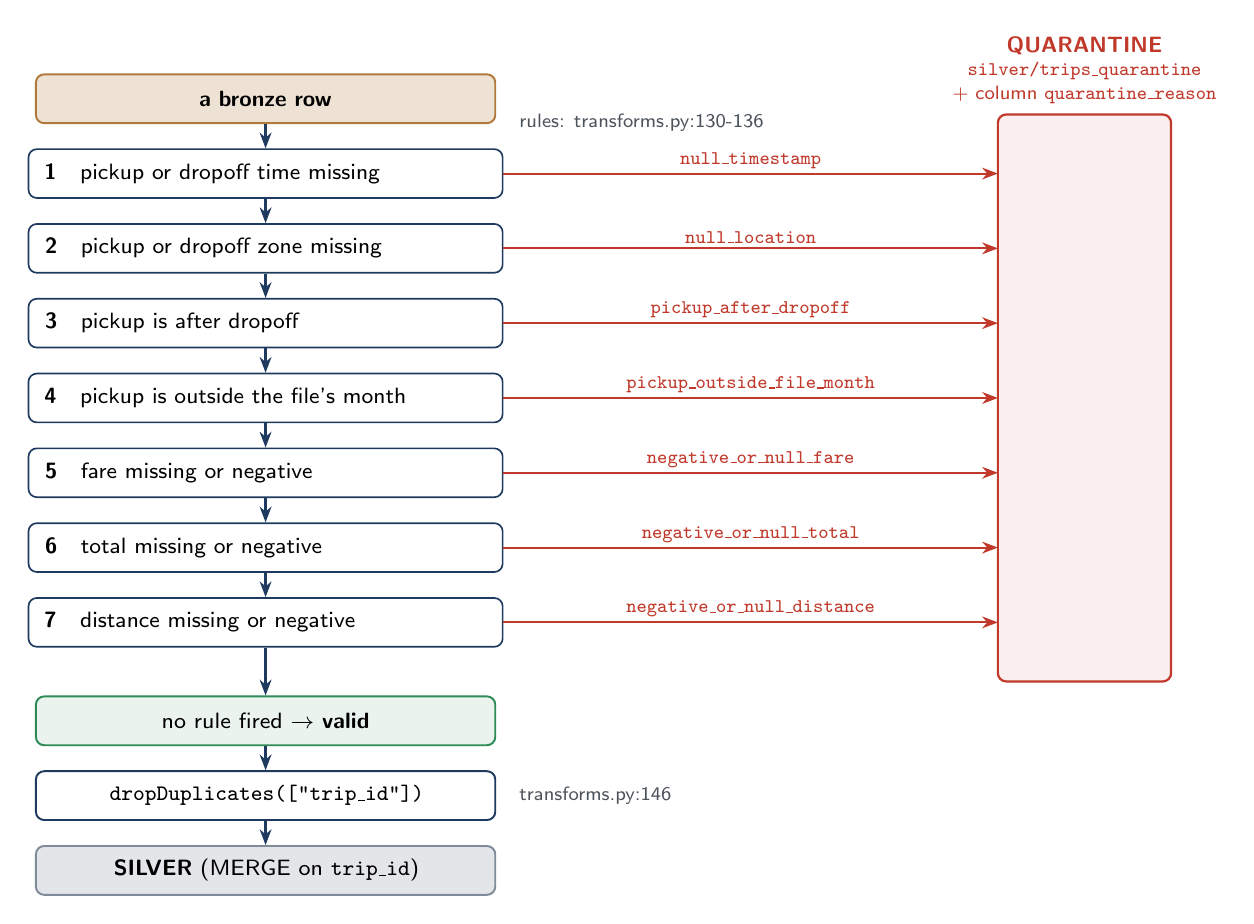
\begin{tikzpicture}[
  font=\footnotesize,
  rule/.style={draw=navy,rounded corners=3pt,fill=white,minimum height=0.62cm,text width=5.6cm,align=left,inner xsep=6pt,line width=0.6pt},
  one/.style={rounded corners=3pt,minimum height=0.62cm,text width=5.6cm,align=center,line width=0.7pt},
  arr/.style={-{Stealth[length=2mm]},line width=0.8pt,color=navy},
  bad/.style={-{Stealth[length=2mm]},line width=0.7pt,color=alert}
]
\node[one,draw=bronze,fill=bronze!22] (in) at (0,0) {\textbf{a bronze row}};
\foreach \i/\t/\r in {
  1/pickup or dropoff time missing/null\_timestamp,
  2/pickup or dropoff zone missing/null\_location,
  3/pickup is after dropoff/pickup\_after\_dropoff,
  4/pickup is outside the file's month/pickup\_outside\_file\_month,
  5/fare missing or negative/negative\_or\_null\_fare,
  6/total missing or negative/negative\_or\_null\_total,
  7/distance missing or negative/negative\_or\_null\_distance} {
  \node[rule] (r\i) at (0,-0.95*\i) {\textbf{\i}\quad\t};
  \draw[bad] (r\i.east) -- node[above,font=\scriptsize\ttfamily,text=alert,inner sep=1.5pt] {\r} (9.3,-0.95*\i);
}
\draw[arr] (in) -- (r1);
\foreach \a/\b in {1/2,2/3,3/4,4/5,5/6,6/7} {\draw[arr] (r\a) -- (r\b);}
\node[draw=alert,fill=alert!8,rounded corners=3pt,minimum width=2.2cm,minimum height=7.2cm,line width=0.8pt] (q) at (10.4,-3.8) {};
\node[align=center,text=alert,anchor=south] at (q.north) {\textbf{QUARANTINE}\\[-1pt]\scriptsize\texttt{silver/trips\_quarantine}\\[-1pt]\scriptsize + column \texttt{quarantine\_reason}};
\node[one,draw=ok,fill=ok!10] (v) at (0,-7.9) {no rule fired $\rightarrow$ \textbf{valid}};
\node[one,draw=navy,fill=white] (dd) at (0,-8.85) {\texttt{dropDuplicates(["trip\_id"])}};
\node[one,draw=silver,fill=silver!22] (sv) at (0,-9.8) {\textbf{SILVER} (MERGE on \texttt{trip\_id})};
\draw[arr] (r7) -- (v); \draw[arr] (v) -- (dd); \draw[arr] (dd) -- (sv);
\node[font=\scriptsize,text=silver!60!black,anchor=west] at (3.1,-8.85) {\f{transforms.py:146}};
\node[font=\scriptsize,text=silver!60!black,anchor=west] at (3.1,-0.3) {rules: \f{transforms.py:130-136}};
\end{tikzpicture}
\figcap{\textbf{Figure 3.} The silver filter (\texttt{quarantine\_reason()}, \f{transforms.py:126-137}). Rules are checked top to bottom; \textbf{the first rule that fails names the reason}, and the row goes to quarantine.}
\end{figure}

\sub{What your output showed}
\begin{lstlisting}[style=out]
[silver] done: 9,417,635 trips, 137,142 quarantined
\end{lstlisting}
About 1.4\,\% of rows (137\,142 of 9\,554\,778) were set aside. That is plausible for raw taxi data (wrong dates, negative fares). We do not know the split per reason yet: see Section~\ref{sec:next}.

\sub{Why it matters for PipeDoctor}
Silver is where most scenarios land: \textbf{3} invalid values (quarantine rules and CHECK constraints), \textbf{8} duplicates after a retry (MERGE on \texttt{trip\_id}), \textbf{11} a column removed upstream (\f{to_silver_candidates} refers to required columns directly, so it fails loudly with an \texttt{AnalysisException}).

% =============================== STEP 6 ===============================
\section{Step 6 \textemdash\ Gold: the business table}
\begin{goal}\textbf{Goal.} Answer a business question quickly: \emph{how many trips and how much revenue per pickup zone per day?}\end{goal}

\sub{Code behind gold}
\codestyle{python}{152}
\begin{lstlisting}
def to_gold(silver: DataFrame) -> DataFrame:
    return silver.groupBy("pickup_date", "pu_location_id").agg(
        F.count("*").alias("trips"),
        F.round(F.sum("total_amount"), 2).alias("revenue"),
        F.round(F.avg("trip_distance"), 3).alias("avg_distance"),
        F.round(F.avg("tip_amount"), 3).alias("avg_tip"),
    )
\end{lstlisting}
\f{gold.py:8-9} reads silver, applies \texttt{to\_gold}, and \textbf{overwrites} the gold table. Gold is cheap to rebuild, so it is simply recomputed from silver every run, never merged.

\sub{What your output showed}
\begin{lstlisting}[style=out]
[gold] done: 20,623 rows
[run_all] green in 567s
\end{lstlisting}
Sanity check: Jan--Mar 2024 is 91 days (2024 is a leap year), and 20\,623 / 91 $\approx$ 227 zones with at least one trip per day. The city has about 265 zone IDs, so this is a sensible number. Each gold row summarises on average 9\,417\,635 / 20\,623 $\approx$ 457 trips.

\sub{Why it matters for PipeDoctor}
Gold is where a silver problem becomes visible to the business (missing days, odd totals). The agent's \texttt{get\_lineage} tool will follow the arrow back: gold $\leftarrow$ silver $\leftarrow$ bronze $\leftarrow$ raw file.

% =============================== STEP 7 ===============================
\section{Step 7 \textemdash\ Run it again (idempotence)}
\begin{goal}\textbf{Goal.} Prove that re-running, which is exactly what happens on a retry, creates no duplicates and changes no numbers.\end{goal}

\sub{Command}
The same \texttt{python -m pipelines.run\_all} as step 4--6.

\sub{Code that makes it safe}
\codestyle{python}{29}
\begin{lstlisting}
    done = already_ingested(spark)
    new = 0
    for path in files:
        name = os.path.basename(path)
        if name in done:
            print(f"[bronze] skip {name} (already ingested)")
            continue
\end{lstlisting}
\f{bronze.py:29-35}: bronze skips any file whose name is already in \texttt{\_source\_file} (\f{bronze.py:17-21}). Silver uses \texttt{whenNotMatchedInsertAll} (\f{silver.py:36-38}): trips that already exist are left alone. Quarantine and gold are \emph{rebuilt}, which is also safe.

\rowcolors{2}{rowgray}{white}
\begin{tabularx}{\textwidth}{@{}>{\bfseries}p{2.2cm}XX@{}}
\toprule
Layer & Run 1 (first time) & Run 2 (re-run) \\
\midrule
Bronze & ingested 3 files, 9\,554\,778 rows & \texttt{skip} $\times$ 3, 0 new, still 9\,554\,778 \\
Silver & table created, 9\,417\,635 trips & MERGE inserted 0, still 9\,417\,635 \\
Quarantine & rewritten, 137\,142 rows & rewritten, 137\,142 rows \\
Gold & 20\,623 rows & recomputed, 20\,623 rows \\
Time & 567\,s & 134\,s \\
\bottomrule
\end{tabularx}

The ${\approx}\,433$\,s difference is roughly the cost of writing the 9.5 million bronze rows (our estimate, not measured separately). The remaining 134\,s is reading, checking and counting.

\begin{pd}\textbf{Why this is the most important step for PipeDoctor.} When a job fails, the standard human reaction is ``just re-run it''. That is only safe if the pipeline is idempotent. Every fix PipeDoctor proposes must keep this property, and scenario~8 (duplicates after a retry) is the test of it.\end{pd}

% =============================== NUMBERS ===============================
\section{Reading the numbers}
\begin{figure}[h]
\centering
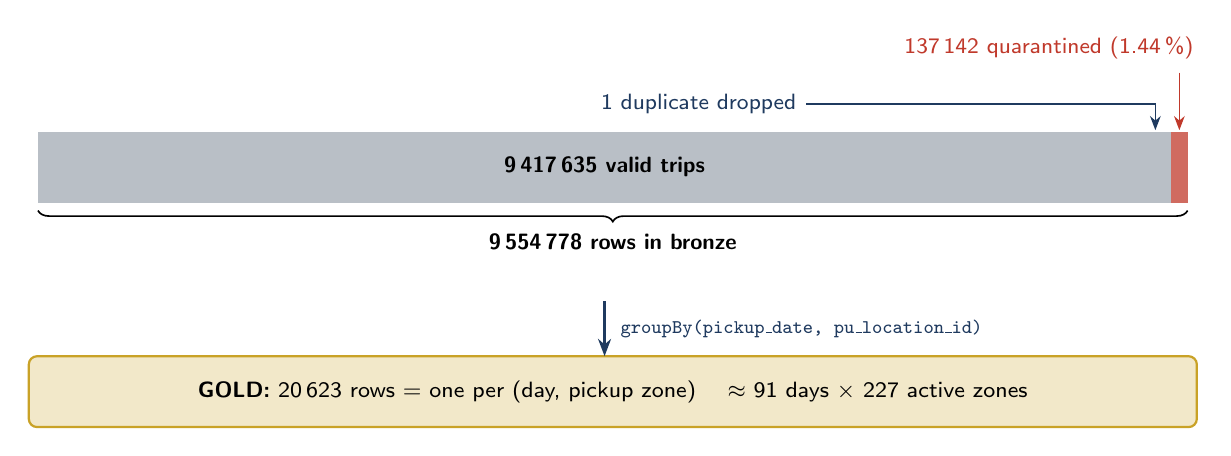
\begin{tikzpicture}[font=\footnotesize]
\def\W{14.6}
\def\tot{9554778}
\pgfmathsetmacro{\wq}{\W*0.0143533}
\pgfmathsetmacro{\ws}{\W-\wq}
\fill[silver!55] (0,0) rectangle (\ws,0.9);
\fill[alert!75]  (\ws,0) rectangle (\W,0.9);
\node at (\ws/2,0.45) {\textbf{9\,417\,635 valid trips}};
\node[anchor=south east,align=right,text=alert] (ql) at (\W+0.2,1.7) {137\,142 quarantined (1.44\,\%)};
\draw[alert,-{Stealth[length=1.8mm]},line width=0.6pt] (\W-\wq/2,1.65) -- (\W-\wq/2,0.92);
\node[anchor=south,align=center,text=navy] (dl) at (\ws-6.0,1.0) {1 duplicate dropped};
\draw[navy,-{Stealth[length=1.8mm]},line width=0.6pt] (dl.east) -| (\ws-0.2,0.92);
\draw[decorate,decoration={brace,amplitude=4pt,mirror},line width=0.6pt] (0,-0.1) -- (\W,-0.1) node[midway,below=5pt] {\textbf{9\,554\,778 rows in bronze}};
\node[draw=gold,fill=gold!25,rounded corners=3pt,minimum height=0.9cm,text width=14.6cm,align=center,line width=0.8pt] (g) at (\W/2,-2.4)
  {\textbf{GOLD:} 20\,623 rows $=$ one per (day, pickup zone) \quad $\approx$ 91 days $\times$ 227 active zones};
\draw[-{Stealth[length=2.2mm]},line width=0.9pt,color=navy] (\ws/2,-1.25) -- node[right,xshift=2pt]{\scriptsize\texttt{groupBy(pickup\_date, pu\_location\_id)}} (\ws/2,-1.95);
\end{tikzpicture}
\figcap{\textbf{Figure 4.} Row accounting from raw to gold. The quarantine slice is drawn to scale; the duplicate is too small to see.}
\end{figure}

\rowcolors{2}{rowgray}{white}
\begin{tabularx}{\textwidth}{@{}Xr>{\raggedright\arraybackslash}p{5.6cm}@{}}
\toprule
Quantity & Rows & Where it is counted \\
\midrule
Bronze & 9\,554\,778 & \f{bronze.py:45} \\
$-$ Quarantined & 137\,142 & \f{silver.py:48} \\
$-$ Duplicates dropped on \texttt{trip\_id} & 1 & deduced, \f{transforms.py:146} \\
\midrule
$=$ Silver & 9\,417\,635 & \f{silver.py:47} \\
\bottomrule
\end{tabularx}

\medskip
\textbf{The ``1''.} The log never prints it, but the logic forces it. Every bronze row goes either to quarantine or to the valid set (\f{transforms.py:143-148}), and the only step that can remove a valid row is \texttt{dropDuplicates}. Since $9\,554\,778 - 137\,142 - 9\,417\,635 = 1$, exactly one row shared its \texttt{trip\_id} with another. The ID hashes eight fields, so these two rows were identical in all eight.

% =============================== NOISE ===============================
\section{Noise versus signal in the log}
Much of the output is harmless chatter. Knowing what to ignore is a real skill for a data engineer, and the first thing PipeDoctor has to learn.

\rowcolors{2}{rowgray}{white}
\begin{longtable}{@{}p{5.2cm}p{2.4cm}p{8.4cm}@{}}
\toprule
Message & Where & Why it is harmless \\
\midrule
\endhead
\texttt{debconf: unable to initialize frontend} & step 1 (\texttt{\#8}) & The build has no interactive terminal; apt falls back to non-interactive mode. \\
\texttt{No JRE found. Skipping Java certificates} & step 1 (\texttt{\#8}) & Order of installation inside apt; the certificates are added a few lines later (\texttt{Adding debian:...}). \\
\texttt{Running pip as the 'root' user} & step 1 (\texttt{\#10}) & We are inside a throw-away container; nothing on your PC is affected. \\
\texttt{hostname resolves to a loopback address} & step 1 (\texttt{\#11}) & Spark picks the container's own IP for local mode. \\
\texttt{Unable to load native-hadoop library} & steps 1 and 4--7 & Spark falls back to pure-Java code. Normal in Docker. \\
\texttt{Truncated the string representation of a plan} & steps 4--7 & Spark only shortens a debug print of a long query plan. \\
\texttt{0 artifacts copied, 3 already retrieved} & steps 4--7 & \textbf{Good news:} the Delta jars come from the image (warm-up, step 1). \\
\bottomrule
\end{longtable}

\begin{watch}\textbf{Signal to look for instead:} a line starting with \texttt{[bronze]}, \texttt{[silver]}, \texttt{[gold]} or \texttt{[run\_all]}; or a Java/Python stack trace ending in an \texttt{Exception}. Those lines are what PipeDoctor will read through \texttt{get\_run\_logs} and \texttt{get\_spark\_error}.\end{watch}

% =============================== NEXT ===============================
\section{What the output does \emph{not} prove yet, and what to do next}\label{sec:next}
\begin{enumerate}[leftmargin=16pt,itemsep=3pt]
\item \textbf{Why were 137\,142 rows quarantined?} The log gives the total, not the reasons. This one command prints the split per rule (we have \emph{not} run it, so treat the result as new information):
\begin{lstlisting}[style=cmd]
docker compose run --rm lakehouse python -c "from pipelines.common.spark import *; s=get_spark(); s.read.format('delta').load(QUARANTINE_PATH).groupBy('quarantine_reason').count().show()"
\end{lstlisting}
\item \textbf{Move the project out of OneDrive.} Your folder is \f{C:\Users\Ayman\OneDrive\Desktop\...}, and \f{data/} now holds the raw files and three Delta tables (likely around a gigabyte). OneDrive will try to sync all of it, which is slow and can lock Delta files. Copy the project to \f{C:\dev\pipedoctor} (the sprint plan's Step 3, Git, needs this too). \f{data/} is already in \f{.gitignore}.
\item \textbf{Look inside the lakehouse.} Open \f{data/lakehouse/bronze/yellow_trips/_delta_log/}: each JSON file is one commit (one per ingested file). This is the \emph{Delta history} that PipeDoctor reads with \texttt{describe\_delta\_history}.
\item \textbf{Next sprint step:} the sprint plan's Step 3, a GitHub repository and CI that runs the same \texttt{pytest} command on every push.
\end{enumerate}

% =============================== LINK TO PD ===============================
\section{How each step connects to PipeDoctor}
\rowcolors{2}{rowgray}{white}
\begin{tabularx}{\textwidth}{@{}c>{\bfseries}p{2.4cm}X@{}}
\toprule
\# & Step & What PipeDoctor will do with it \\
\midrule
1 & Image & Run candidate fixes in the \emph{same} environment (\texttt{run\_sandbox\_job}). \\
2 & Download & Scenario 4: a late file is escalated to a human, not patched. \\
3 & Tests & The \emph{Validate} step: a fix that breaks one of the 8 tests is rejected. \\
4 & Bronze & Scenarios 1--2: schema drift and type change (\texttt{BRONZE\_CONTRACT}, \texttt{mergeSchema}). \\
5 & Silver & Scenarios 3, 8, 11: invalid values, duplicates after a retry, column removed upstream. \\
6 & Gold & Where the business notices; \texttt{get\_lineage} walks back to the cause. \\
7 & Re-run & Every fix must preserve idempotence, otherwise a retry creates duplicates. \\
\bottomrule
\end{tabularx}

\section{Cheat sheet: the five commands}
\begin{lstlisting}[style=cmd]
# step 1  (only again if Dockerfile or requirements.txt change)
docker compose build

# step 2  download the data
docker compose run --rm lakehouse python scripts/download_taxi_data.py --start 2024-01 --months 3

# step 3  unit tests
docker compose run --rm lakehouse python -m pytest pipelines/tests -q

# steps 4-6  bronze, silver, gold   (run it twice = step 7)
docker compose run --rm lakehouse python -m pipelines.run_all

# bonus  open a shell inside the container
docker compose run --rm lakehouse bash
\end{lstlisting}
Rule of thumb: \textbf{code changes need no rebuild} (the project folder is mounted), \textbf{Dockerfile or requirements changes do}.

\end{document}
